% Figure 15 -- Seiberg-Witten graph for an irregular + a regular singularity
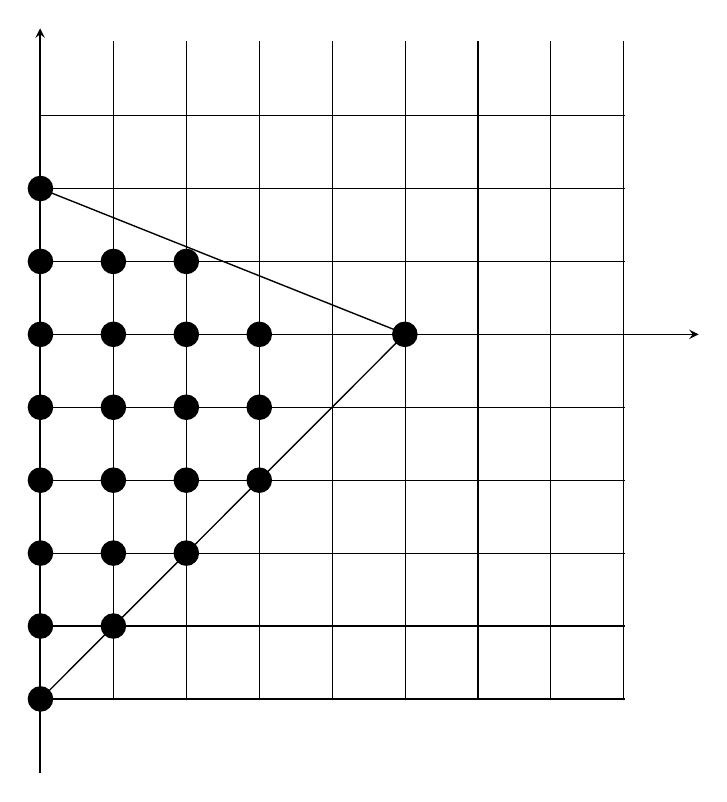
\begin{tikzpicture}[x=1pt,y=1pt,scale=1.05,transform shape,>=stealth,line width=0.5pt]
  \def\u{25.095}
  % ---- grid ----
  \foreach \i in {0,...,8} {\draw[line width=0.4pt] (66.5,28.4) ++(\i*\u,0) -- ++(0,227.1);}
  \foreach \j in {-5,...,3} {\draw[line width=0.4pt] (65.9,{154.4+\j*\u}) -- (267.8,{154.4+\j*\u});}
  % ---- axes ----
  \draw[->] (65.9,154.4) -- (293,154.4);
  \draw[->] (66.4,3.4) -- (66.4,259.7);
  % ---- the two Newton-polygon edges ----
  \draw (66.6,28.9) -- (191.9,154.4);
  \draw (65.9,204.8) -- (192.6,154.3);
  % ---- marked points ----
  \foreach \j in {2,1,0,-1,-2,-3,-4,-5} {\fill (66.5,{154.4+\j*\u}) circle[radius=4.4pt];}
  \foreach \j in {1,0,-1,-2,-3,-4}     {\fill (91.6,{154.4+\j*\u}) circle[radius=4.4pt];}
  \foreach \j in {1,0,-1,-2,-3}        {\fill (116.7,{154.4+\j*\u}) circle[radius=4.4pt];}
  \foreach \j in {0,-1,-2}             {\fill (141.8,{154.4+\j*\u}) circle[radius=4.4pt];}
  \fill (191.9,154.4) circle[radius=4.4pt];
\end{tikzpicture}
